\begin{tikzpicture}[scale=0.8,rotate=237]
    
    % Define los puntos de un triángulo
    \tkzDefPoint(0,0){A}
    \tkzDefPoint(5,0){B}
    \tkzDefPoint(3,3){C}
    
    % Dibuja el triángulo
    \tkzDrawPolygon(A,B,C)

    %\tkzDrawPoints(A,B,C)
    \tkzLabelPoint[above](A){$D$}
    \tkzLabelPoint[left](B){$E$}
    \tkzLabelPoint[right](C){$F$}
    
    % Marca cada lado con barritas
    \tkzMarkSegment[mark=|](A,B)
    \tkzMarkSegment[mark=||](B,C)
    \tkzMarkSegment[mark=|||](A,C)
\end{tikzpicture}